\chapter{Saga atómsins}

\section{Hið agnarsmáa kemur í skömmtum}

Sagan af hinu agnarsmáa hefst hjá forngríska heimspekingnum, Demókrítusi (460-370 f.~Kr), sem staðhæfði fystur manna að allt efni samanstæði af litlum ókljúfanlegum einingum sem að hann kallaði frumeindir eða atóm. Síðan gerðist því miður ekkert í atómsögunni í meira en þúsund ár og hugmyndir Demókrítusar féllu smátt og smátt í gleymsku. Það var kannski aðallega af því að kenningar Demókrítusar voru í beinni mótsögn við kenningar Aristótalesar (sem er og var miklu vinsælli heimspekingur heldur en Demókrítus, en það segir kannski allt sem segja þarf um heimspekinga). Söguna tók síðan upp að nýju árið 1797 hjá breska efnafræðingnum John Dalton. Hann hafði tekið eftir því að þegar að maður blandar saman tveimur mismunandi efnum (t.d. nitri og súrefni) til þess að búa til nýja efnablöndu þá getur maður fengið margar mismunandi útkomur eftir því í hvaða hlutföllum maður blandar saman efnunum. Til dæmis ef að maður tekur \SI{140}{g} af nitri og bætir við \SI{80}{g} af súrefni þá fær maður hláturgas eða tvínituroxíð ($\ce{N_2O}$). Hinsvegar ef að maður tvöfaldar magnið af súrefni og bætir við \SI{160}{g} í staðinn þá fær maður nituroxíð ($\ce{NO}$). Loks ef maður fjórfaldar upprunalega magnið af súrefni og setur \SI{320}{g} af súrefni þá fær maður niturtvíoxíð ($\ce{NO_2}$). Það eru semsagt einhver tengsl við heiltölurnar $1$:$2$:$4$ (og um leið og við sjáum tengsl við heiltölurnar þá eigum við að hugsa um einhver skammtatengsl!). \\

Þessi uppgötvun Daltons kann að virðast augljóst fyrir skólagengnum nútímamanni sem hefur þegar lært atómkenninguna og veit að það er ekki hægt að blanda frumefnum saman í hvaða hlutföllum sem er (til dæmis er ekki til $\ce{NO_{\sqrt{2}}}$ því það er ekki hægt að tengja $\sqrt{2}$ súrefnisatóm við hvert nituratóm). En á þeim tíma þegar Dalton setti þessar athuganir fram þá var þetta afar skrítin niðurstaða sem stangaðist á við upplifun samtímamannsins af náttúrunni. Til þess að setja þetta í samhengi, þá var þetta svolítið eins og að maður væri með uppskrift að piparkökum og myndi síðan hundraðfalda magnið af pipar (eins og bakaradrengurinn í Dýrunum í Hálsaskógi) og í staðinn fyrir að fá mjög vondar piparkökur þá fengi maður dásemdar vínabrauðslengju. \\

Með þessari uppgötvun Daltons fóru hjólin að snúast því nú var hægt að nýta sér þessa skammtahugmynd til þess að mæla atómmassa tiltekinna frumefna (í hlutfalli við hvert annað). Þá skilgreindu menn léttasta frumefnið, vetni, þannig að það hefði atómmassann $\SI{1}{u}$ (þá var auðvitað ekki þekkt að $\SI{1}{u} = \SI{1.67e-27}{kg}$ þar að auki sem að það er ólíklegt að Dalton hafi notað kílóið þar sem að það hafði fyrst verið skilgreint tveimur árum fyrr, árið 1795). Þannig var hægt að ákvarða að súrefni hefði atómmassann $\SI{16}{u}$ með því að vigta það í samanburði við vetni í efnasamsetningunni $\ce{H2O}$. Reyndar hélt Dalton sjálfur lengi vel að vatn væri efnasambandið $\ce{HO}$ sem gaf honum þá röngu niðurstöðu að hlutföllin væru þannig að súrefni hefði atómmassann \SI{5.5}{u} (hann gerði þar að auki algebruvillu!) sem sýnir kannski helst að þrátt fyrir þessa stórmerku uppgötvun Daltons þá var enn langt í land hvað varðaði heilstæða atómkenningu. Dalton birti síðan árið 1805 töflu sem sýndi massa mismunandi frumefna í hlutfalli við massa vetnis. Það má segja að þetta hafi í einhverjum skilningi verið fyrsta lotukerfið. Þar með hafði atómkenning Demókrítusar verið endurvakin og fyrsti vísirinn að mólhugtakinu verið lagður (mólið er skilgreint sem fjöldi kolefnisatóma í \SI{12}{g} af kolefni en það væri alveg eins hægt að skilgreina það eins og Dalton gerði sem fjölda vetnisatóma í \SI{1}{g} af vetni).  \\

Með frumeindamassakenningu Daltons fóru menn að uppgötva ný efni og bæta í töflu Daltons. Árið 1863 var búið að bera kennsl á 56 frumefni og greina frumeindamassa þeirra. Það var hinsvegar ekki fyrr en árið 1867 sem að rússneski efnafræðingurinn Dmitri Mendelejev bjó til hið hefðbundna lotukerfi sem að við þekkjum í dag. Sagan segir að lotukerfið hafi birst honum í draumi: \\

\begin{tcolorbox}

\iduck{I saw in a dream a table where all elements fell into place as required. Awakening, I immediately wrote it down on a piece of paper, only in one place did a correction later seem necessary.} \\

\vspace{-0.3cm}
\raggedleft{- \textbf{Dmitri Mendelejev, 1867}}
\end{tcolorbox}

\begin{comment}
\begin{figure}[H]
    \centering
    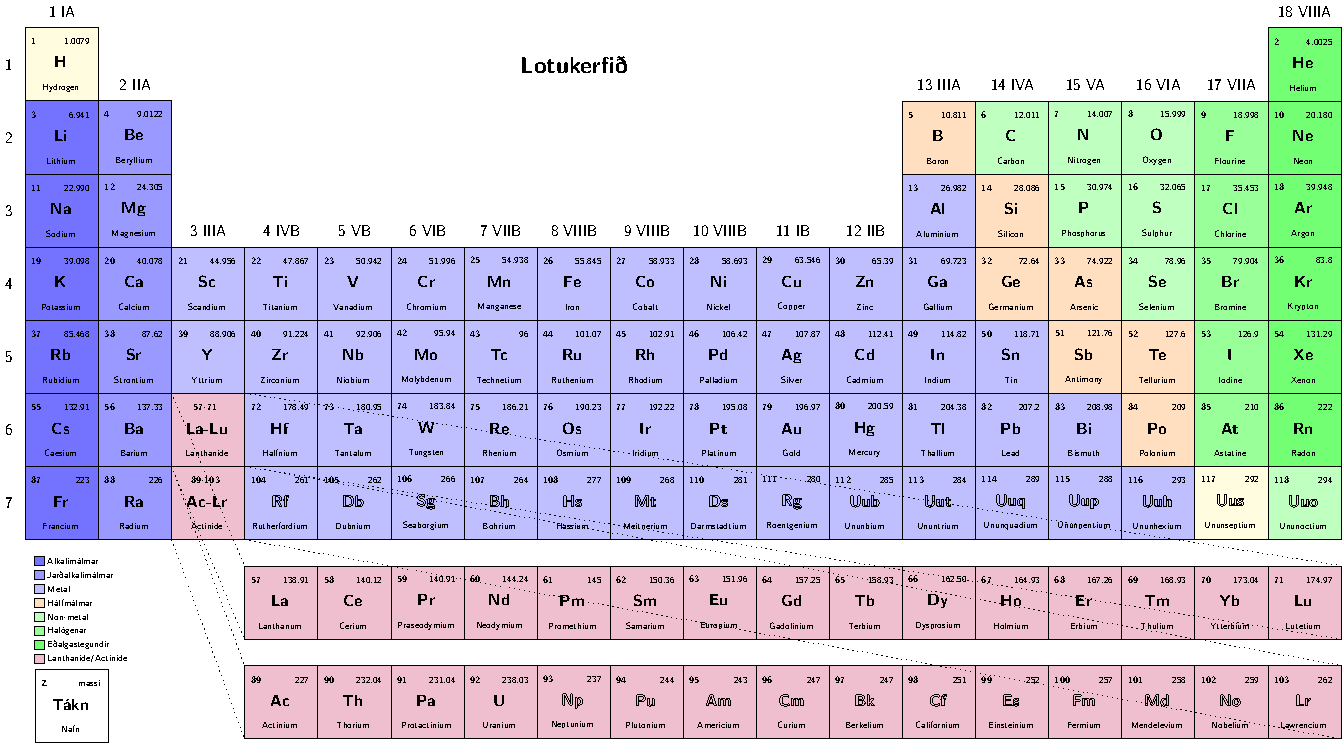
\includegraphics[width=.5\textwidth]{figures/lotukerfi2.pdf}
\end{figure}
\end{comment}

Eftir að Mendelejev hafði safnað saman efnunum í samræmi við efnaeiginleika þeirra tók hann eftir að það voru göt í töflunni. Hann dró þá ályktun að það ætti eftir að uppgötva frumefni sem að myndu fylla í skarðið. Þannig tókst honum að spá fyrir um tilvist þriggja nýrra efna,  German, (\ce{Ge}), Gallín, (\ce{Ga}) og Skandín (\ce{Sc}). Það sem meira var þá spáði hann fyrir um frumeindamassa þeirra ásamt ýmsum efnaeiginleikum þeirra. German fannst síðan árið 1875, Skandín árið 1879 og Gallín árið 1886 og öll smellpössuðu inn í götin í lotukerfi Mendelejevs eins og hann hafði spáð fyrir um. Þetta átti ekki eftir að vera síðasta skiptið í mannkynssögunni þar sem að fræðimanni tókst að spá fyrir um tilvist öreindar (vitið þér enn eða hvað?). \\

Með frumeindamassakenningu Daltons hafði verið hægt að raða frumefnunum með frumeindamassa $A$ í sætaröð með sætistölu $Z$. Til dæmis hafði vetni frumeindamassa $A = 1$ og sætistölu $Z = 1$ en súrefni hafði frumefnamassa $A = 16$ og sætistölu $Z = 8$. En lotukerfi Mendelejevs benti á að það væru enn leyndardómar sem væri hægt að afhjúpa. Hvað var það sem að stjórnaði þessum efnaeiginleikunum sem að Mendelejev gat spáð fyrir um?  Var það kannski rétt hjá Aristótalesi eftir allt saman, að þessi ókljúfanlegu atóm, voru hugsanlega kljúfanleg og höfðu innri byggingu sem gat útskýrt þessa efnaeiginleika og þessi mynstur í lotukerfinu? Það er kannski í einhverjum skilningi 
í svona vangaveltum sem að hjarta eðlisfræðinnar liggur. Við þurfum stöðugt að vera að bera kennsl á mynstur í náttúrunni og reyna að finna leiðir til þess að útskýra þessi mynstur. Það vill bara oftast svo óheppilega til að um leið og ein útskýring er fundin þá uppgötva menn nýjar tengingar á öðrum sviðum sem valda því að við berum kennsl á enn fleiri og flóknari mynstur og vítahringurinn endurtekur sig í sífellu! \\

\section{Thomson uppgötvar rafeindina}

Það var síðan árið 1897 sem að Breski eðlisfræðingurinn og nóbelsverðlaunahafinn, J.J.~Thomson\footnote{J.J. Thomson var doktorsleiðbeinandi fyrir 8 aðra nóbelsverðlaunahafa (6 í eðlisfræði og 2 í efnafræði).}, uppgötvaði rafeindina og þar með hafði hið ókljúfanlega atóm verið klofið!  Við skulum fjalla aðeins um það hvernig að J.J. Thomson uppgötvaði rafeindina en til þess að skillja aðdraganda þess þá þurfum við að fara aðeins aftur á bak í sögunni. Við þurfum að fara aftur til ársins 1838 til Michael Faradays (já það er maðurinn á bak við hið alræmda spanlögmál). Faraday langaði til þess að skilja hvernig og hvort að það væri hægt að leiða rafmagn í gegnum gas. Hann tók því tvær plötur (í plötuþétti) og setti þær inn í glerpípu og lækkaði þrýstinginn á gasinu. Hann tengdi síðan plöturnar við jafnspennugjafa. Honum til mikillar undrunar þá byrjaði gasið að glóa með fjólubláum lit! Þessir geislar voru kallaðir katóðugeislar\footnote{Orðin katóða og anóða eru tekin úr forngrísku og merkja annars vegar lækkun og hinsvegar lyfting eða hækkun} því þeir komu frá neikvæðu plötu plötuþéttisins (hægt er að athuga það með því að setja eitthvað fyrir og sjá hvorum meginn skugginn fellur). Nú á dögum vitum við að þessir svokölluðu katóðugeislar eru ekkert annað en straumur af rafeindum (það var einmitt uppgötvun J.J. Thomson). Þegar að rafeidnirnar lenda í árekstrum við gasið þá örvast gassameindirnar upp í hærra orkustig en þegar að þær falla aftur niður í grunnástand sitt þá geislast orkumismunur ástandanna út sem ljós. Í rauninni má líta á sem svo að þessi glerpíputilraun Faradays hafi verið fyrsti öreindahraðallinn. Næstu árin voru menn að betrumbæta glerpíputilraun Faradays.

\begin{figure}[H]
    \centering
    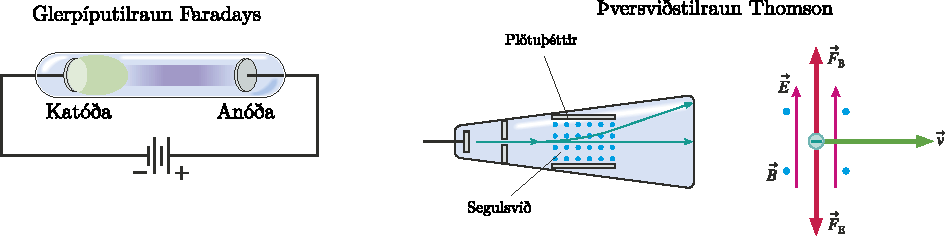
\includegraphics[]{figures/jjthomson.pdf}
\end{figure}

Snildarhugmynd J.J. Thomson var síðan að setja inn einsleitt rafsvið og segulsvið inn í miðjuna á glerpípunni (með plötuþétti og spólu). En á þeim tíma var þekkt að rafsegulkraftarnir sem að hlaðnar agnir finna fyrir vegna rafsviðsins og segulsviðsins eru gefnir með:
\begin{align*}
    F_E = qE, \hspace{0.5cm} \text{og} \hspace{0.5cm} F_B = qvB
\end{align*}
En í tilviki Thomsons þá stillti hann tækinu sínu þannig upp að katóðugeislinn ferðaðist beint á milli platna plötuþéttisins. Þá gat hann ályktað að:
\begin{align*}
    F_B = F_E \implies qE = qvB \implies v = \frac{E}{B}.
\end{align*}
Eftir að hann hafði síað út hraða eindanna í katóðugeislanum þá sendi hann geislan áfram í einsleitt segulsvið (sjá massagreininn í fyrirlestri 6). Hann gat síðan mælt geisla hringhreyfingarinnar sem að eindir katóðugeislans ferðuðust með. Þá fékk hann samkvæmt hringhreyfingunni að:
\begin{align*}
    m\frac{v^2}{r} = qvB \implies \frac{q}{m} = \frac{v}{rB}.
\end{align*}
Það var engin leið fyrir Thomson til þess að ákvarða hleðslu né massa eindanna í katóðugeislanum. En hann gat mælt hlutfallið milli hleðslu eindnana og massa þeirra: $\frac{q}{m}$. Gildið sem að hann fékk í tilraunninni fyrir katóðugeislana var:
\begin{align*}
    \frac{e}{m_e} = \SI{1.76e11}{C/kg}.
\end{align*}
En þetta var miklu hærra hlutfall heldur en allt annað sem var þekkt á þessum tíma! Næst hæsta hlutfallið sem var þekkt á þessum tíma var fyrir vetnisjónina $\ce{H+}$ (betur þekkt sem róteind í dag en róteindin hafði ekki verið uppgötvuð á þeim tíma) en þar var hlutfallið:
\begin{align*}
    \frac{e}{m_p} = \SI{9.59e7}{C/kg}
\end{align*}
Hlutfallið í þversviðstilraun Thomsons var því um það bil 1836 sinnum hærra heldur en næsthæsta þekkta hlutfallið á þeim tíma! Það kannski ber að nefna á þessum tímapunkti að menn vissu ekki endilega að katóðugeislinn samanstæði af rafeindum og því var tvennt í stöðunni: Annað hvort samanstóð katóðugeislinn af eindum með mjög mikla hleðslu eða af eindum með mjög lítinn massa (tvær leiðir til þess að gera hlutfallið $\frac{q}{m}$ stórt). Flest virti benda til þess að það væri massinn sem væri mjög lítill (því menn höfðu áttað sig á því að hleðsla væri skömmtuð stærð þó að þeir hefðu ekki ákvarðað minnstu skammtastærðina á hleðslunni, þ.e. grunnhleðsluna~$e = \SI{1.602e-19}{C}$). Eina leiðin hinsvegar til þess að skera út um það hvort það væri mjög stór hleðsla eða mjög lítill massi sem að eindirnar í katóðugeislanum hefðu þá þurftu menn samt að finna leið til þess að mæla annað hvort eitt og sér! En það var einmitt þessi skammtahugmynd um grunnhleðsluna sem að leiddi menn á sporið. Það var nefnilega frekar auðvelt á þessum tíma að ákvarða heildarhleðsluna á einu móli af sameindum svo í rauninni þá var helsta vandamálið að ákvarða Avogadrosartöluna, $N_A$\footnote{Reyndar má sjá með gaslögmálinu að $PV = nRT$ þar sem $n$ er mólfjöldinn og það var frekar auðvelt að mæla gasfastann $R$ (með því að gera tilraun með t.d.~\SI{1}{móli} af gasi þar sem rúmmáli er t.d.~haldið föstu $V = V_0$ og gera graf af $P$ sem fall af $T$). En gasfastinn tengist Avogadrosartölunni og Boltzmann fastanum samkvæmt $R = k_B N_A$ svo það var þar með jafngilt að ákvarða Boltzmann-fastann $k_B$.} (þekkt gildi í dag er $N_A = \SI[per-mode=fraction]{6.022e23}{\frac{1}{mól}}$. Fyrsta mælingin á Avogadrosartölunni\footnote{Reyndar vilja sumir eigna franska lækninum Johann Chrysostomus Magnenus (1646) heiðurinn. En sagan segir að hann hafi ákvarðað Avogadrosartöluna með Fermi-tilraun. Hann kveikti á ilmkerti í tómri kirkju og mældi tímann sem það tók fyrir ilminn að berast hinum meginn í kirkjuna. Út frá því hversu langan tíma það tók fyrir hann að finna lyktina af ilmkertinu gat hann metið stærð Avogadrosartölunnar út frá rúmmáli kirkjunnar.} hafði verið gerð árið 1865 af Johann Josef Loschmidt (gildið sem að hann fékk var reyndar \SI{4.0e22}{\frac{1}{mól}} sem er nokkuð fjarri þekktu gildi í dag).\footnote{Kannski er það smá útúrdúr en í einni af Annus Mirablis greinum Einsteins (1905) sem fjallar um Brown-hreyfingu þá sýnir Einstein hvernig er hægt að ákvarða Boltzmann-fastann (og þar með gasfastann) mjög nákvæmlega þar að auki sem að hann sýnir hvernig er hægt að ákvarða stærð frumeinda.} Þetta gaf Thomson leið til þess að meta massa eindanna í katóðugeislanum og færa rök fyrir því að eindirnar í katóðugeislunum hefðu mun minni massa heldur en léttasta eindin sem var þekkt á þeim tíma. Hann var þar með búinn að finna öreind sem var smærri heldur en allar þekktar frumeindir þess tíma. \\

\section{Olíudropatilraun Millikan og Fletchers}

Það tók hinsvegar smá tíma fyrir menn að samþykkja þessa niðurstöðu Thomsons um nýja öreind sem væri smærri heldur en frumeindirnar. Það var í rauninni ekki fyrr en árið 1909 þegar Millikan og Fletcher\footnote{Robert Millikan var doktorsleiðbeinandi Harvey Fletchers og birti ekki nafn Fletchers á grein þeirra um olíudropatilraunina. Þetta gerði það að verkum að Millikan hlaut nóbelsverðlaunin einn árið 1923 fyrir mælinguna á grunnhleðslunni þegar hann hefði líklegast átt að deila verðlaununum með Fletcher.} framkvæmdu svokallaða olíudropatilraun sem gaf einfalda leið til þess að mæla grunnhleðsluna, $e$. Uppstillingin fyrir olíudropatilraunina var frekar einföld í sjálfu sér. Þeir settu spennumun $\Delta V = Ed$ á milli tveggja platna í plötuþétti og slepptu síðan olíudropum með hleðslu $q$ og massa $m$ á milli platna plötuþéttisins.

\begin{figure}[H]
    \centering
    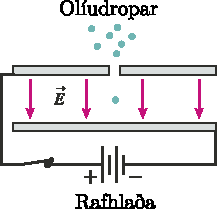
\includegraphics{figures/oliudropar.pdf}
\end{figure}

Eina leiðin fyrir dropana til þess að haldast kyrrir í lausu lofti var ef að rafkrafturinn var jafn stór og þyngdarkrafturinn, þ.e.~ef
\begin{align*}
    mg = qE \implies q = \frac{mg}{E} = \frac{mgd}{\Delta V}.
\end{align*}
Þar sem $\Delta V$ var spennumunurinn á milli platna plötuþéttisins. Þetta var auðveldi hlutinn í olíudropatilrauninni. Erfiði hlutinn í tilraun Millikans og Fletchers var síðan að ákvarða massa olíudropanna sem að þeir höfðu komið þarna fyrir á milli platnanna. En málið var að olíudroparnir þeirra voru alveg gríðarlega smáir. Þvermál olíudropanna var af stærðargráðunni \SI{}{\mu m} svo það var hægt að sjá þá í stækkunargleri en það var nánast ómögulegt að fá nákvæmt mat á stærð þeirra (óvissan hefði gert tilraunina ómarktæka). En þar sem að olíudroparnir voru svo gríðarlega smáir þá var loftmótsstaðan sem að droparnir fundu fyrir gríðarlega mikil en það þýddi að þegar slökkt var á rafsviðinu þá varð loftmótsstaðan svo gríðarlega mikil að olíudroparnir byrjuðu nánast samstundis að falla með föstum lokahraða (því loftmótsstöðukrafturinn og þyngdarhröðunin eru jafn stórir í fallinu). Með því að mæla tímann sem að það tók fyrir eindirnar að fall niður að plötum plötuþéttisins var hægt að meta lokahraða eindanna og þar með massa þeirra. Til þess að útskýra þetta aðeins nánar þá var þekkt að loftmótsstöðukrafturinn sem að verkaði á dropana (að því gefnu að þeir væru kúlulaga með geisla $r$) var gefinn með:
\begin{align*}
    F_{\!_\text{loftmótsstaða}} = 6\pi \eta rv
\end{align*}
þar sem $\eta$ táknar seigju vökvans (í þessu tilviki loft með $\eta_{\text{loft}} = \SI{18.5e-6}{Pa.s}$). Með því að skoða hvenær kraftajafnvægi næst þá höfum við að:
\begin{align*}
    0 = ma = mg - 6\pi \eta rv \implies v_{\text{lok}} = \frac{mg}{6\pi \eta r} 
\end{align*}
En hægt var að tengja massa dropanna við eðlismassann samkvæmt $m = \rho V_{\text{dropi}} = \frac{4 \pi \rho}{3}r^3$ þannig að:
\begin{align*}
    v_{\text{lok}} = \frac{mg}{6\pi \eta r} = \frac{2}{9} \frac{\rho g}{\eta} r^2 \implies r = 3\sqrt{\frac{\eta v_{\text{lok}}}{2 \rho g}}.
\end{align*}
En þar með gátu Millikan og Fletcher ályktað að:
\begin{align*}
    q = \frac{mgd}{\Delta V} = \frac{4 \pi \rho r^3 g d}{3 \Delta V} = 18 \pi \frac{d}{\Delta V} \sqrt{\frac{\eta^3 v^3_{\text{lok}}}{2 \rho g}}.
\end{align*}

Eftir að hafa haft svona mikið fyrir þessari útleiðslu þá er frekar fyndið að Millikan og Fletcher notuðu vitlaust gildi á seigju loftsins í útreikningum sínum! Richard Feynman hafði eftirfarandi um málið að segja:

\begin{tcolorbox}
\iduck{We have learned a lot from experience about how to handle some of the ways we fool ourselves. One example: Millikan measured the charge on an electron by an experiment with falling oil drops, and got an answer which we now know not to be quite right. It's a little bit off because he had the incorrect value for the viscosity of air. It's interesting to look at the history of measurements of the charge of an electron, after Millikan. If you plot them as a function of time, you find that one is a little bit bigger than Millikan's, and the next one's a little bit bigger than that, and the next one's a little bit bigger than that, until finally they settle down to a number which is higher.
Why didn't they discover the new number was higher right away? It's a thing that scientists are ashamed of—this history—because it's apparent that people did things like this: When they got a number that was too high above Millikan's, they thought something must be wrong—and they would look for and find a reason why something might be wrong. When they got a number close to Millikan's value they didn't look so hard. And so they eliminated the numbers that were too far off, and did other things like that.} \\

\vspace{-0.3cm}
\raggedleft{- \textbf{Richard Feynman, 1974}}
\end{tcolorbox}

\section{Gullþynnutilraun Rutherfords}

Sama ár og Millikan og Fletcher framkvæmdu olíudropatilraunina sína þá uppgötvuðu Ernest Rutherford\footnote{Rutherford hafði sjálfur verið doktorsnemi hjá J.J. Thomson og hafði fengið Nóbelsverðlaunin í efnafræði 1908, árið áður en gullþynnutilraunin var framkvæmd.}og doktorsnemar hans, Hans Geiger og Ernest Mardsen, kjarna frumeindanna með gullþynnutilrauninni. Þetta er án efa ein merkasta og frægasta tilraun mannkynssögunnar. Niðurstaða tilraunarinnar var svo sláandi og algjörlega í mótsögn við allt sem að menn þekktu á þeim tíma. \\

Uppstillingin í gullþynnutilraun Rutherfords var eftirfarandi. Geislavirkri uppsprettu (nánar um geislavirkni aðeins síðar) var staðsett fyrir aftan blývegg með litlu gati. Blýveggurinn átti að sjá til þess að $\alpha$-geislunin frá geislavirku uppsprettunni beindist aðeins beint í gegnum gullþynnuna. Við vitum í dag að $\alpha$-geislun er ekkert annað en geisli af helínjónum $\ce{He^++}$ sem samanstendur af tveimur róteindum og tveimur nifteindum, en það var ekki þekkt á þeim tíma. Fyrir aftan gullþynnuna var síðan sinksúlfat skjár sem gaf frá sér lítinn ljósblossa þar sem $\alpha$-agnirnar lentu á skjánum.

\begin{figure}[H]
    \centering
    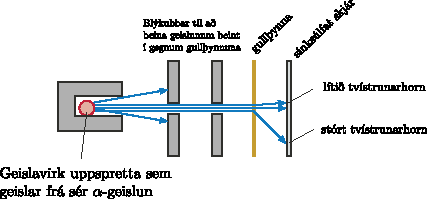
\includegraphics{figures/rutherford-gold.pdf}
\end{figure}

Rutherford hafði beðið doktorsnemana sína Geiger og Mardsen um að framkvæma þessa tilraun svo að þeir gætu staðfest atómlíkan þess tíma sem var kennt við J.J. Thomson lærimeistara Rutherfords. Atómlíkan Thomsons kallaðist rúsínukökulíkanið (líka stundum plómubúðingslíkanið) og sagði að atómið væri eins og rúsínukaka þar sem að rúsínurnar voru rafeindirnar sem voru jafndreifðar í jákvætt hlaðna kökudeginu. Ástæðan fyrir því að þetta var viðtekið á þeim tíma var að Thomson hafði sýnt fram á að rafeindir væru minni heldur en frumeindirnar og menn vissu að flestar frumeindir voru óhlaðnar (jafn mikið af róteindum og rafeindum) en einfaldasta leiðin (rakvél Occams) sem að þeim datt í hug til þess að útskýra þetta var einmitt ef að litlu róteindirnar væru jafndreifðar inni í jákvætt hlaðna atóminu. Það sem að Rutherford, Geiger og Mardsen bjuggust við var að þeir myndu alltaf fá örlítil tvístrunarhorn (ekki alveg núll en þeir bjuggust við því að stærsta mögulega tvístrunarhornið væri um það bil \ang{0.02} eða svo gott sem núll). Niðurstaðan þeirra var satt best að segja fáránleg í samanburði við atómlíkan THomsons. Ekki nóg með það að tvístrunarhornin voru stærri heldur en það sem að þeir bjuggust við heldur gerðist það í um það bil 1 af hverjum 8000 mælingum að $\alpha$-agnirnar endurvörpuðust aftur að uppsprettunni! Þær höfðu þá snúið við um \ang{180} gráður) sem var fáránlegt! Rutherford hafði sjálfur eftirfarandi um niðurstöðuna að segja:


\begin{tcolorbox}

\iduck{It was quite the most incredible event that has ever happened to me in my life. It was almost as incredible as if you fired a 15-inch shell at a piece of tissue paper and it came back and hit you.} \\

\vspace{-0.3cm}
\raggedleft{- \textbf{Rutherford, 1909}}
\end{tcolorbox}

Hvernig var hugsanlega hægt að útskýra þessa niðurstöðu? Það er eiginlega smá kómískt að það hafi verið Rutherford sjálfur sem að útskýrði fræðilega hvernig stæði á þessari tilraunaniðurstöðu í gullþynnutilrauninni. En Rutherford er af mörgum talinn færasti verklegi eðlisfræðingur allra tíma (Michael Faraday er hugsanlega sá eini sem stóð honum fremri). Reyndar er Rutherford frægur fyrir að hafa haft mikla óbeit á fræðilegri eðlisfræði og eftirfarandi tilvitnun lýsir kannski skoðunum hans á fræðilegum eðlisfræðingum hvað best:

\begin{tcolorbox}

\iduck{How can a fellow sit down at a table and calculate something that would take me six months to measure in a laboratory?\phantom{}} \\

\vspace{-0.3cm}
\raggedleft{- \textbf{Rutherford, 1909}}
\end{tcolorbox}

En Rutherford áttaði sig á því hvernig væri hægt að útskýra þessa tilraunaniðurstöðu á fræðilegan hátt. Árið 1911 setti hann fram atómlíkan þar sem að hann kom með þá tilgátu að í miðjunni á atóminu væri kjarni sem bæri jákvæða hleðslu $+Q$. Hann sýndi enn fremur að ef að $\alpha$-ögnin hefði massa $m$, upphafshraða $v_0$ og væri skotið í áttina að kjarnanum úr fjarlægð $b$ (sjá myndina hér fyrir neðan fyrir nánari útskýringu) þá myndi tvístrunarhorn $\alpha$-geislans njóta jöfnunnar:
\begin{align*}
    b = \frac{qQ}{2\pi \epsilon_0 mv_0^2} \cot(\frac{\theta}{2}).
\end{align*}

\begin{figure}[H]
    \centering
\begin{tikzpicture}
    \draw[thick, fill=black] (1.2,0) circle (0.1cm);
    \draw[thick, fill=black] (-3,1) circle (0.05cm);
    \draw[dashed] (-3,0) -- (4.5,0);
    \draw[dashed] (0,0) -- (3,3);
    \draw[dashed] (1.2,0) -- (4.2,3);
    \draw[Stealth-Stealth] (2,2) -- (2.7,1.5);
    \draw[Stealth-Stealth] (-2.5,1) -- (-2.5,0);
    \draw[-Stealth] (-2.85,1.3) -- (-2.2,1.3);
    \draw[dashed] (-3,1) -- (4.5,1);
    \node at (-2.3,0.5) {$b$};
    \node at (2.6,2) {$b$};
    \draw[thick, -Stealth] (-3,1) .. controls (0,1) and (1,1) .. (3,3);
     \draw (1.7,0) arc (0:46:0.5);
     \node at (1.875,0.25) {$\theta$};
     \node at (1.4,-0.3) {$Q$};
     \node at (-3.2,1.25) {$q$};
     \node at (-2.7, 1.55) {$\vec{v}_0$};
     \node at (3.2, 3.1) {$\vec{v}_f$};
\end{tikzpicture}
\end{figure}
Þar með sjáum við að ef $b = 0$ þá verður $\cot(\frac{\theta}{2}) = 0$ svo $\theta = \ang{180}$ og ögnin endurkastast beint til baka. Rutherford sýndi þar að auki að líkurnar á því að ögnin myndi tvístrast um horn $\theta$ væru gefnar með:
\begin{align*}
    \sigma(\theta) = \frac{Q^2q^2}{4mv^2v_0^2\sin^4(\frac{\theta}{2})}
\end{align*}
Þannig gat hann staðfest hlutfallið 1/8000 fyrir fullkomið endurkast í samræmi við mælingar þeira Geiger og Mardsen.

Tvístrunarhorn Rutherfords og atómkjarnakenning hans gerðu það að verkum að nú voru menn komnir með einfalda leið til þess að mæla fjölda róteinda í kjarnanum. Það sem meira var þá gerði þetta þeim kleift að meta stærðina á kjarnanum sem um það bil af stærðargráðunni \SI{e-15}{m} í samanburði við \SI{e-10}{m} fyrir stærð atómsins\footnote{Rutherford notaði viðlíkinguna að kjarninn væri eins og fluga í dómkirkju.}. Með þessari vitneskju tókst Breska eðlisfræðingnum Henry Moseley\footnote{Sagan segir að Moseley hefði líklegast hlotið nóbelsverðlaunin 1916 hefði hann ekki látist 1915 í orrustunni við Gallipoli í fyrri heimsstyrjöldinni. Hann var þá 27 ára.} (sem var líka einn af doktorsnemum Rutherfords) að ákvarða $7$ ný frumefni út frá sætistölunni, $Z$, með röngengeislamælingum (x-ray). \\

\section{Chadwick uppgötvar nifteindina}

Það kann kannski að virðast undarlegt sagnfræðilega - en það liðu síðan rúmlega 20 ár þar til að nifteindin var uppgötvuð árið 1932. Það kann að virðast augljóst í dag því hvert mannsbarn veit að heildarfjöldi nifteinda í kjarnanum er $A-Z$ þar sem $A$ er frumeindamassinn og $Z$ er sætistala frumefnisins. Það eitt og sér ætti að vera nóg til þess að fá eðlisfræðinga í það minnsta til þess að leita að nýrri kjarneind! En nei, svona getur eðlisfræðin vafist fyrir manni! Því fræðilegir eðlisfræðingar halda lengi fast í fallegar kenningar þó svo að þær séu rangar. Í þessu tilviki vildu þeir ekki gefast upp á rúsínukökulíkani Thomsons svona einfaldlega. En þetta var ekki einfaldlega útaf því að þeir voru að reyna að halda í gamla, bilaða kenningu. Það var reyndar mjög margt sem að benti til þess að svo væri! Helstu rökin sem að menn höfðu fyrir þessu rúsínukökulíkani fyrir kjarnan var $\beta$-geislun. En þegar að geislavirk efni senda frá sér $\beta$-geislun þá senda efnin út rafeindir úr kjarnanum og sætistalan lækkar. Hvernig gat rafeindinni verið skotið út úr kjarnanum nema ef að hún hafði verið þar til að byrja með? Kenningin á þeim tíma var þess vegna að inni í kjarnanum væru orkuríkar rafeindir á sveimi til þess að halda kjarnanum saman. Það var því á þeim tíma engin þörf fyrir nýja kjarneind eins og nifteindina til þess að útskýra eitt eða neitt. Menn töldu sig þegar hafa uppgötvað allt sem hægt var að vita um atómkjarnan! \\

Kannski var önnur ástæða þess hvað það tók langan tíma að uppgötva nifteindina að það var svo margt annað í gangi í eðlisfræði á þessum tíma. Fremstu eðlisfræðingar þess tíma voru að leggja línurnar að almennu afstæðiskenningunni, skammtafræði og skammtasviðsfræði. Það var enginn tími né hagur af því að vinna að rannsóknum í kjarneðlisfræði (Ó, hvað tímarnir áttu eftir að breytast!). Reyndar var skammtafræðin nú þegar á þessum tíma farin að benda á galla í þessu ranga, viðtekna rúsínukökukjarnalíkani en það var enginn að leita að þessum mótsögnum og þar með var enginn búinn að taka eftir þeim á þessum tíma! Reyndar var hugmyndin svo rótgróin að Enrico Fermi\footnote{Já, þetta er hinn eini sanni Enrico Fermi sem átti eftir að meta stærð fyrstu kjarnorkusprengjunnar með blaðsnifsum.} og Franco Rasetti skrifuðu grein 1926 þar sem að þeir sýndu fram á að þetta líkan samræmdist ekki kenningum um spuna. Þeir ályktuðu út frá niðurstöðunni að spunahugmyndin væri röng (en ekki öfugt!). Það sem meira var þá var uppgötvunin á nifteindinni eiginlega bara slys! Hún var algjörlega ótengd allri þessari nýju eðlisfræði sem var verið að þróa á þessum tíma. Hún fannst eiginlega bara óvart! \\

Árið 1930 höfðu Walter Bothe og Herbert Becker framkvæmt tilraun þar sem að þeir skutu $\alpha$-geislum að beryllín uppsprettu. Þeir tóku eftir því að við þetta þá geislaði beryllín uppsprettan frá sér nýrri geislun, sem að þeir héldu í fyrstu að væru $\gamma$-geislun (það reyndist ekki vera rétt). Tilraunin var endurtekin af Iréne Curie\footnote{Iréne Curie var dóttir Marie Curie og Pierre Curie. Það gleymist stundum í umræðunni að Iréne Curie og Fréderic Joliot hlutu einnig Nóbelsverðlaunin í efnafræði 1935. Marie Curie og Pierre Curie hlutu nóbelsverðlaunin í eðlisfræði saman (ásamt Antoine Henri Becquerel) árið 1903. Marie Curie hlaut síðan nóbelsverðlaunin í efnafræði árið 1911 (Pierre lést árið 1906). Þar með státar Curie-fjölskyldan sig af 5 nóbelsverðlaunum!} og Fréderic Joliot eiginmanni hennar. Þau ályktuðu (ranglega) eins og Bothe og Becker að efnahvarfið væri:
\begin{align*}
    \ce{^{9}_{4}Be + ^{4}_{2}$\alpha$ -> ^{13}_{6}C + $\gamma$}
\end{align*}
Ítalski eðlisfræðingurinn Ettore Majorana á að hafa sagt þegar hann frétti þessa niðurstöðu þeirra:

\begin{tcolorbox}

\iduck{What fools! They have disovered the neutral proton, and they do not recognise it!\phantom{}} \\

\vspace{-0.3cm}
\raggedleft{- \textbf{Ettore Majorana, 1931}}
\end{tcolorbox}


En þetta voru frábærar fréttir fyrir James Chadwick (enn einn doktorsnemi Rutherfords) en hann hafði verið að leita að öreind eins og nifteindinni í mörg ár! Í stuttri grein sem að Chadwick birti árið 1932 þá sýndi hann fram á að þessi geislun sem að Bothe-Becker-Curie-Joliot höfðu greint frá beryllín uppsprettunni gat ómögulega verið $\gamma$-geislun því hann sýndi hver mesta hugsanlega orkan sem $\gamma$-geislinn gæti haft (og sú tala var lægri heldur en orka geislanna sem að þau höfðu greint). Þar með ályktaði hann að hér væri ný eind uppgtötvuð og hið rétta kjarnahvarf væri:
\begin{align*}
    \ce{^{9}_{4}Be + ^{4}_{2}$\alpha$ -> -> ^{12}_{6}C + ^{1}_{0}n}
\end{align*}

Hingað til held ég að sagan okkar af atóminu hafi fjallað um atriði sem að þið teljið ykkur þekkja ágætlega, þ.e.~að atómið samanstendur af rafeindum, róteindum og nifteindum þar sem að róteindirnar og nifteindirnar eru pakkaðar þétt saman í örlitlum kjarna af stærðargráðunni \si{fm} og rafeindirnar eru á sveimi í kringum kjarnan í órafjarlægð (hlutfallslega) þannig að stærð atómsins er af stærðargráðunni \si{\AA}. Þetta er plánetulíkan Rutherfords\footnote{Oft líka kennt við Bohr en tæknilega séð var Joseph Larmor fyrstur til þess að stinga upp á plánetulíkani af atóminu.} af atóminu og er eflaust enn þann dag í dag það atómlíkan sem að almúgamaðurinn kannast hvað best við (þið hafið síðan hugsanlega lært um líkindadreifingu rafeinda í efnafræði en meira um það síðar). Það er eiginlega frekar magnað að þetta plánetulíkan sé enn þann dag í dag kennt í menntakerfinu. Því þetta var bókstaflega bara atómlíkanið í 100 daga! Því aðeins 100 dögum eftir að Chadwick greindi frá því að hann hefði uppgötvað nifteindina þá tilkynntu samstarfsfélagar hans við Cavendish tilraunastofuna í Cambridge að þeir hefðu fundið jáeindina. Stuttu eftir það byrjuðu ótal margar nýjar öreindir að koma fram á sjónarsviðið. Reyndar voru öreindirnar svo margar að Enrico Fermi á að hafa sagt:

\begin{tcolorbox}

\iduck{If I could remember the names of all those particles, I’d be a botanist.} \\

\vspace{-0.3cm}
\raggedleft{- \textbf{Enrico Fermi, 1953}}
\end{tcolorbox}

En áður en að við kynnum þessar nýju öreindir til sögunnar (sem að þið hafið líklegast aldrei heyrt um!) þá skulum við staldra við og rífa plánetulíkanið af atóminu algjörlega í sundur og sína hvers vegna það er ekki nógu gott og hvaða mótsagnir það felur í sér! Því maður hefur ekki skilið eðlisfræðikenningu nógu vel fyrr en að maður getur sýnt að hún sé röng! Ætli það sé ekki kannski markmiðið í eðlisfræði eftir allt saman? Að afsanna flóknar kenningar og búa til nýjar flóknari kenningar fyrir aðra til þess að afsanna! \\


\section{Staðallíkanið}

\begin{tcolorbox}

\iduck{Three quarks for Muster Mark! \\
Sure he hasn't got much of a bark \\
And sure any he has it's all beside the mark.} \\

\vspace{-0.3cm}
\raggedleft{- \textbf{Finnegans Wake eftir James Joyce, 1939}}
\end{tcolorbox}

Árið 1932 höfðu menn komist að því að allt efni samanstæði af atómum og að öll atóm samanstæðu af örlitlum kjarna af þétt pökkuðum róteindum og nifteindum. Umhverfis kjarnan voru rafeindir á sveimi. Á þeim tíma voru þetta einu eindirnar sem voru þekktar sem voru smærri heldur en atómið. Ef að lotukerfið tekur saman helstu eiginleika frumeindanna þá gætum við þess vegna smíðað einfalt lotukerfi sem að útskýrir hvernig að frumeindirnar eru búnar til:

\begin{figure}[H]
    \centering
    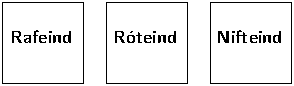
\includegraphics[width=.5\textwidth]{figures/lotukerfi3.pdf}
\end{figure}


En nú þegar menn höfðu klofið atómið og séð að það samanstóð af róteindum, nifteindum og rafeindum þá datt mönnum það snilldarráð í hug að reyna að kljúfa þessar nýju eindir líka! Því eins og Aristótales hafði sagt þá var alltaf hægt að komast dýpra! Hingað til hefur mönnum ekki tekist að kljúfa rafeindina. Hinsvegar tókst mönnum að kljúfa bæði róteindina og nifteindina niður í svokallaða kvarka\footnote{Orðið kvarki var valið af Gell-Mann og er tekið úr eftirfarandi } árið 1964. Þar að auki fundu menn nýja öreind árið 1956 sem kallast fiseind. Fiseindin er óhlaðin og er miklu léttari heldur en hinar efniseindir staðallíkansins\footnote{Í langan tíma var talið að fiseindin hefði engan massa. En í dag er talið að hún hafi massa af stærðargráðunni $\SI{e-37}{kg}$ eða rúmlega milljón sinnum minni massa heldur en rafeindin.}. Róteindin samanstendur af tveimur upp kvörkum og einum niður kvarka á meðan að nifteindin samanstendur af tveimur niður kvörkum og einum upp kvarka. Til þess að þetta geti gengið upp þá þarf upp kvarkinn að hafa hleðslu $+\frac{2}{3}$ en niður kvarkinn hleðslu $-\frac{1}{3}$. Þá sjáum við einmitt að hleðsla róteindarinnar verður $(\frac{2}{3} + \frac{2}{3} - \frac{1}{3} = +1)$ en hleðsla nifteindarinnar verður $(-\frac{1}{3} - \frac{1}{3} + \frac{2}{3} = 0)$.

\begin{figure}[H]
    \centering
    \subfloat{{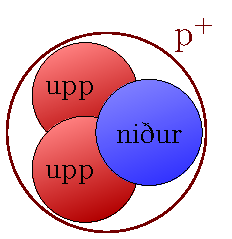
\includegraphics[scale = 1]{figures/up-quark.pdf}
         }}%
    \qquad
    \subfloat{{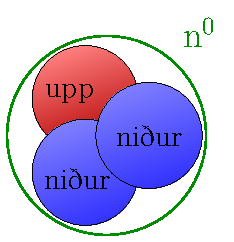
\includegraphics[scale = 1]{figures/nidur-quark.pdf} }}%
\end{figure}


Þar með varð lotukerfið fyrir minnstu byggingareiningar efnisheimsins eftirfarandi:

\begin{figure}[H]
    \centering
    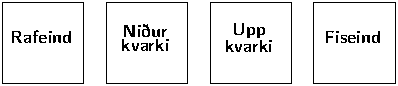
\includegraphics[width=.5\textwidth]{figures/lotukerfi4.pdf}
\end{figure}

Í einhverjum skilningi má segja að þetta sé lotukerfið okkar í dag og að við ættum að stoppa núna áður en að þið hættið að skilja boffs. En nú fyrst fer sagan okkar að verða áhugaverð! \\

Af einhverjum undarlegum ástæðum sem að engum hefur tekist enn þann dag í dag að skilja þá ákváð náttúran að endurtaka þetta mynstur tvisvar (og aðeins tvisvar) í viðbót. Náttúran afritaði þessar eindir nema gerði þær bara aðeins þyngri (en annars hafa þær svipaða eiginleika). Til dæmis eru afritin af rafeindinni kallaðar mýeind ($\mu$) og táeind $(\tau)$ og þær hafa massa:
\begin{align*}
    m_{\mu} \approx 207 m_e, \hspace{1cm} m_\tau \approx 3483 m_e.
\end{align*}

Þegar að við afritum efniseindirnar fáum við (talan táknar massa eindanna sem margfeldi af massa rafeindar):


\begin{figure}[H]
    \centering
    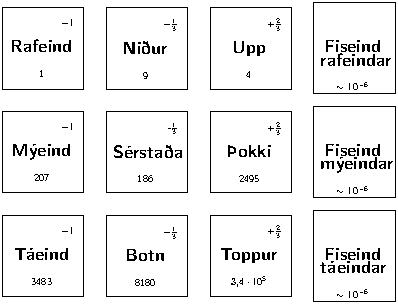
\includegraphics[width=.5\textwidth]{figures/lotukerfi5.pdf}
\end{figure}

Hver lína í þessu lotukerfi kallast \textbf{kynslóð}. Allar kynslóðirnar samanstanda af fjórum eindum: Einni sem að líkist rafeindinni og tilheyrandi fiseind hennar og tveimur kvörkum. Allar eindirnar í fyrsta dálkinum hafa hleðslu $-1$. Allir kvarkarnir í öðrum dálkinum hafa hleðslu $-\frac{1}{3}$, allir kvarkarnir í þriðja dálknum hafa hleðslu $+\frac{2}{3}$ og allar fiseindirnar eru óhlaðnar. \\

Það er margt sem að eðlisfræðingar hafa komist að í tengslum við mynstrin í þessu nýja lotukerfi. Til dæmis getum við útskýrt hvers vegna hleðslur eindanna þurfa að vera nákvæmlega þær sem þær eru. Það sem meira er, ef við myndum einn daginn uppgötva rafeindareftirhermu úr fjórðu kynslóðinni þá myndum við samstundis vita að það væru til tveir kvarkar og tilheyrandi fiseind þar að auki í fjórðu kynslóðinni. Hinsvegar, þá er einnig margt sem að við skiljum ekki í þessu lotukerfi. Til dæmis bendir flest allt til þess að það séu ekki fleiri kynslóðir heldur en einungis þessar þrjár.\footnote{Helstu rökin sem að fólk færir fyrir því er að í fjórðu kynslóðinni þá væru tilheyrandi fiseindir ekki lengur léttar heldur væru þær þvert á móti þungar og líklegast \SI{e10}{} sinnum þyngri en þær fiseindir sem að við þekkjum.} Við skiljum ekki af hverju það eru einungis þrjár kynslóðir af efniseindum en ekki t.d.~14 eða 30. Það dularfyllsta í þessu öllu saman er að við skiljum ekki mynstrin sem að ákvarða massa eindanna. Þetta er semsagt niðurstaðan: Það eru $12$ efniseindir til og allt efni er búið til úr samsetningu af þessum $12$ efniseindum.\footnote{Hver þeirra á síðan tilheyrandi andeind svo í rauninni eru efniseindirnar 24.} \\

En þetta er í rauninni bara efnishelmingur staðallíkansins (við munum bráðlega kynna hinn helming staðallíkansins). Á þessum tímapunkti vaknar upp arargrúi af íðorðum sem að eðlisfræðingar nota í fagmáli sínu til þess að almúginn geti ekki skilið staðallíkanið almennilega. Til dæmis hafa þessar 12 efnisagnir fengið samheitið \textbf{fermíeindir}\footnote{Tæknilega séð er skilgreiningin á fermíeind sú að það séu allar þær eindir sem hafa hálf-tölu spuna eins og til dæmis $\frac{1}{2}, \frac{3}{2}, \ldots$} (til heiðurs ítalska eðlisfræðingnum Enrico Fermi). Fermíeindirnar tólf skiptast í sex kvarka (quark) og sex \textbf{létteindir} (lepton). Stundum segjum við síðan að kvarkarnir hafi \textbf{bragð} (flavour). Til dæmis væri þokki bragð á kvarka). Allar eindir sem eru samsettar úr þremur kvörkum kallast \textbf{þungeindir} (baryon). Til dæmis eru róteindin (tveir upp, einn niður) og nifteindin (einn upp, tveir niður) dæmi um þungeindir.

\newpage

En nú komum við að seinni hluta staðallíkansins, en hann samanstendur af \textbf{bóseindum}\footnote{Paul Dirac gaf eindunum það nafn til heiðurs indverska eðlisfræðingnum Satyendra Nath Bose sem hlaut aldrei nóbelinn.} sem eru stundum líka kallaðar \textbf{kraftberar}. En það eru þær eindir sem að gera efniseindunum (fermíeindunum) kleift að tala saman og finna fyrir hver annarri. Þið þekkið nú þegar eina bóseind en það er \textbf{ljóseindin} sem að miðlar rafsegulkraftinum (með öðrum orðum eru ljóseindir kraftberar rafsegulkraftsins). Við ættum síðan að nefna á þessu stigi kraftana fimm. Það kemur í ljós að það eru eindir sem að miðla kraftinum. Svokallaðar kraftberar:

\begin{itemize}
    \item Þyngdarkrafturinn: Þyngdarkrafturinn er frekar sérstakur. Almenna afstæðiskenning Einsteins sýnir að þyngdarsviðið er í rauninni tímarúmið sjálft. Gárur í tímarúminu eru kallaðar þyngdarbylgjur og tilheyrandi kraftberar, svokallaðar, þyngdareindir, hafa aldrei verið mældar.
    
    \item Rafsegulkrafturinn: Ljóseindir, $\gamma$, bera rafsegulkraftinn.
    
    \item Sterki kjarnakrafturinn: Límeindir, $g$, bera sterka kjarnakraftinn.
    
    \item Veiki kjarnakrafturinn: $W$, $Z^-$ og $Z^+$ bóseindirnar bera veika kjarnakraftinn.
    
    \item Higgs-krafturinn: Higgs-eindin, $H$, ber Higgs-kraftinn. Higgs-sviðið sem gefur ögnum massa.
\end{itemize}



Við skulum nú setja fram staðallíkanið í allri sinni dýrð:

\begin{figure}[H]
    \centering
    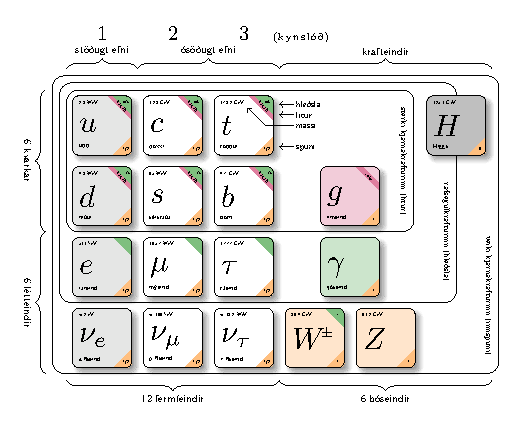
\includegraphics[width=.7\textwidth]{figures/standardmodel.pdf}
\end{figure}

\begin{figure}[H]
    \centering
    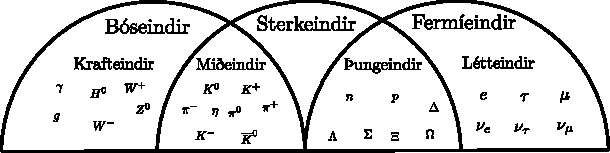
\includegraphics[scale = 1.25]{figures/jargon-diagram.pdf}
    \caption{Vennmynd sem sýnir flokkun öreinda.}
\end{figure}

\newpage